\newpage
\section{RAG (Retrieval-Augmented Generation) Workflow}
\label{sec:rag}

Das Herzst\"uck von EduShelf ist die RAG-Pipeline: Anstatt das LLM allein auf sein allgemeines Wissen zu st\"utzen, wird jede Benutzeranfrage zun\"achst dazu genutzt, relevante Textabschnitte aus den hochgeladenen Dokumenten abzurufen. Diese Abschnitte werden dann als \textit{Kontext} in den Prompt eingef\"ugt, bevor das LLM zur Antwort aufgefordert wird. Dies reduziert Halluzinationen und erm\"oglicht präzise sowie dokumentspezifische Antworten.

\subsection{System\"ubersicht und Datenfluss}
Das folgende Diagramm visualisiert den vollst\"andigen Anfrage-Antwort-Zyklus im RAG-System und zeigt, wie die verschiedenen Services zusammenarbeiten.

\begin{figure}[h]
    \centering
    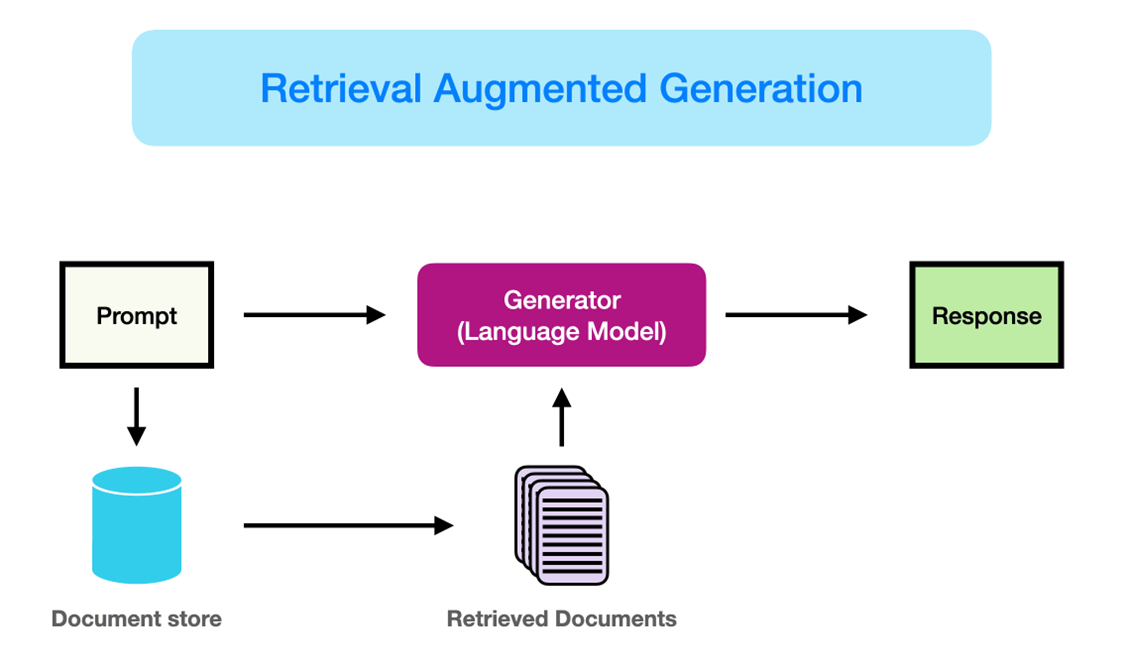
\includegraphics[width=\textwidth]{img/rag_system.png}
    \caption{Architekturdiagramm des RAG-Systems in EduShelf}
    \label{fig:rag_system}
\end{figure}

Der Datenfluss bei einer Benutzeranfrage l\"asst sich in f\"unf klar abgegrenzte Schritte gliedern:
\begin{enumerate}
    \item \textbf{Anfrage \& Intent-Erkennung:} Der \texttt{ChatController} empf\"angt die Nachricht des Nutzers und leitet sie an den \texttt{ChatService} weiter. Dieser \"ubergibt sie zuerst an den \texttt{IntentDetectionService}.
    \item \textbf{Vektorielle Suche (Retrieval):} Basierend auf dem erkannten Intent ruft der \texttt{RetrievalService} die semantisch relevantesten \texttt{DocumentChunks} aus der PostgreSQL/pgvector-Datenbank ab.
    \item \textbf{Kontext-Aufbereitung:} Der \texttt{PromptGenerationService} kombiniert den Konversationsverlauf, die abgerufenen Chunks und die aktuelle Frage zu einem Prompt.
    \item \textbf{LLM-Inferenz:} \"Uber das Microsoft Semantic Kernel SDK wird der Prompt an das lokal laufende Ollama-LLM gesendet.
    \item \textbf{Antwort \& Persistenz:} Die generierte Antwort wird in der Datenbank als \texttt{ChatMessage} gespeichert und an den Client zur\"uckgegeben.
\end{enumerate}

\subsection{Schritt 1: Intent-Erkennung (\texttt{IntentDetectionService})}
\label{subsec:intent}

Bevor eine semantische Suche stattfindet, muss das System verstehen, \textit{was} der Nutzer m\"ochte. Der \texttt{IntentDetectionService} sendet die Benutzeranfrage an das LLM mit einem speziellen System-Prompt, der das Modell anweist, eine strukturierte JSON-Antwort zu liefern:

\begin{lstlisting}[language={[Sharp]C}, caption={Intent-Erkennung via LLM in IntentDetectionService.cs}]
var chatHistory = new ChatHistory();
chatHistory.AddSystemMessage(
    _configuration.GetValue<string>("AIService:Prompts:Intent")
    ?? "Identify the intent.");
chatHistory.AddUserMessage(userInput);

var result = await chatCompletionService.GetChatMessageContentAsync(chatHistory);
var cleanedJson = JsonHelper.ExtractJson(result.Content ?? string.Empty);
var intent = JsonSerializer.Deserialize<Intent>(cleanedJson,
    new JsonSerializerOptions { PropertyNameCaseInsensitive = true })
    ?? new Intent { Type = "question", DocumentName = null };
\end{lstlisting}

Das \texttt{Intent}-Objekt enth\"alt zwei Felder:
\begin{itemize}
    \item \texttt{Type}: Klassifiziert die Anfrage als \texttt{"question"}, \texttt{''summarize"}, \texttt{"flashcards"} oder \texttt{"quiz"}.
    \item \texttt{DocumentName}: Falls der Nutzer explizit ein Dokument nennt (z.B. \glqq{}Erkl\"are mir Kapitel 3 aus Physik.pdf\grqq{}), wird der Dateiname hier extrahiert.
\end{itemize}

Dieser Schritt ist entscheidend für den weiteren Prozess: Anstatt starr immer dieselbe RAG-Pipeline zu durchlaufen, wird die Antwort-Strategie dynamisch an den jeweiligen Kontext angepasst.

\subsection{Schritt 2: Semantische Suche (\texttt{RetrievalService})}
\label{subsec:retrieval}

Der \texttt{RetrievalService} ist f\"ur die Beschaffung der relevanten Dokumentenabschnitte zust\"andig. Er implementiert dabei eine zweistufige Strategie:

\subsubsection{Prim\"are Suche: Name-basiertes Matching}
Falls der Intent einen \texttt{DocumentName} enth\"alt, sucht der Service direkt nach Chunks, deren \"ubergeordnetes Dokument diesen Namen tr\"agt. Dies erfolgt \"uber einen PostgreSQL-spezifischen, gro\ss{}-/kleinschreibungsunabh\"angigen Vergleich (\texttt{ILike}):

\begin{lstlisting}[language={[Sharp]C}, caption={Dokumenten-spezifische Suche in RetrievalService.cs}]
var chunks = await _context.DocumentChunks
    .Include(dc => dc.Document)
    .Where(dc => dc.Document.UserId == userId &&
           (EF.Functions.ILike(dc.Document.Title, intent.DocumentName) ||
            EF.Functions.ILike(dc.Document.Title,
            documentNameWithoutExtension)))
    .ToListAsync();
\end{lstlisting}

\subsubsection{Fallback: Semantische Vektorsuche}
Wenn kein Dokumentname angegeben wurde oder keine Treffer gefunden wurden, wird eine semantische Suche \"uber alle Chunks des Nutzers durchgef\"uhrt. Die Anfrage wird in einen Embedding-Vektor umgewandelt und mit allen gespeicherten Chunk-Vektoren per L2-Distanz verglichen:

\begin{lstlisting}[language={[Sharp]C}, caption={Embedding-basierte Vektorsuche in RetrievalService.cs}]
var promptEmbedding = await _embeddingGenerator.GenerateAsync(userInput);
var k = GetDynamicK(userInput); // 5, 10 oder 20 Chunks

return await _context.DocumentChunks
    .Include(dc => dc.Document)
    .Where(dc => dc.Document.UserId == userId)
    .OrderBy(dc => dc.Embedding.L2Distance(new Vector(promptEmbedding.Vector)))
    .Take(k)
    .ToListAsync();
\end{lstlisting}

Der Wert $k$ (Anzahl der zur\"uckgegebenen Chunks) ist dynamisch: Bei kurzen Anfragen (unter 10 W\"ortern) werden $k=5$, bei mittleren $k=10$ und bei komplexen Anfragen (\"uber 30 W\"orter) $k=20$ Chunks abgerufen.

\subsection{Schritt 3: Prompt-Aufbau (\texttt{PromptGenerationService})}
\label{subsec:prompt}

Der \texttt{PromptGenerationService} baut eine vollst\"andige \texttt{ChatHistory} auf, die drei Elemente enth\"alt:
\begin{itemize}
    \item Eine \textbf{System-Instruktion}, die das Verhalten des LLMs grundlegend steuert.
    \item Den \textbf{bisherigen Konversationsverlaif} der aktuellen Chat-Sitzung (f\"ur kontextsensitive Folgefragen).
    \item Die \textbf{aktuelle Benutzeranfrage}, angereichert mit dem abgerufenen Dokumentenkontext.
\end{itemize}

\begin{lstlisting}[language={[Sharp]C}, caption={Prompt-Konstruktion in PromptGenerationService.cs}]
// Kontext aus Chunks zusammenstellen und auf Token-Limit kuerzen
foreach (var chunk in relevantChunks) {
    contextText.AppendLine($"[{chunk.Document.Title}] {chunk.Content}");
}
contextString = _tokenService.Truncate(contextString, contextLengthLimit);

// Finale Benutzernachricht mit eingebettetem Kontext
finalUserMessage.AppendLine($"[Context from Documents]:\n{contextString}\n");
finalUserMessage.AppendLine($"[User Question]: {userInput}");
chatHistory.AddUserMessage(finalUserMessage.ToString());
\end{lstlisting}

Ein zentrales Element ist die \textbf{Token-Limitierung} durch den \texttt{ITokenService}. Um das Kontextfenster des LLMs (Standardmäßig: 4096 Tokens) nicht zu \"uberschreiten, werden die Chunks vor der \"Ubergabe tokenisiert und pr\"azise abgeschnitten (\textit{Smart Truncation}). Dies verhindert API-Fehler und stellt sicher, dass die semantisch n\"achsten Chunks priorisiert werden.

\begin{figure}[H]
    \centering
    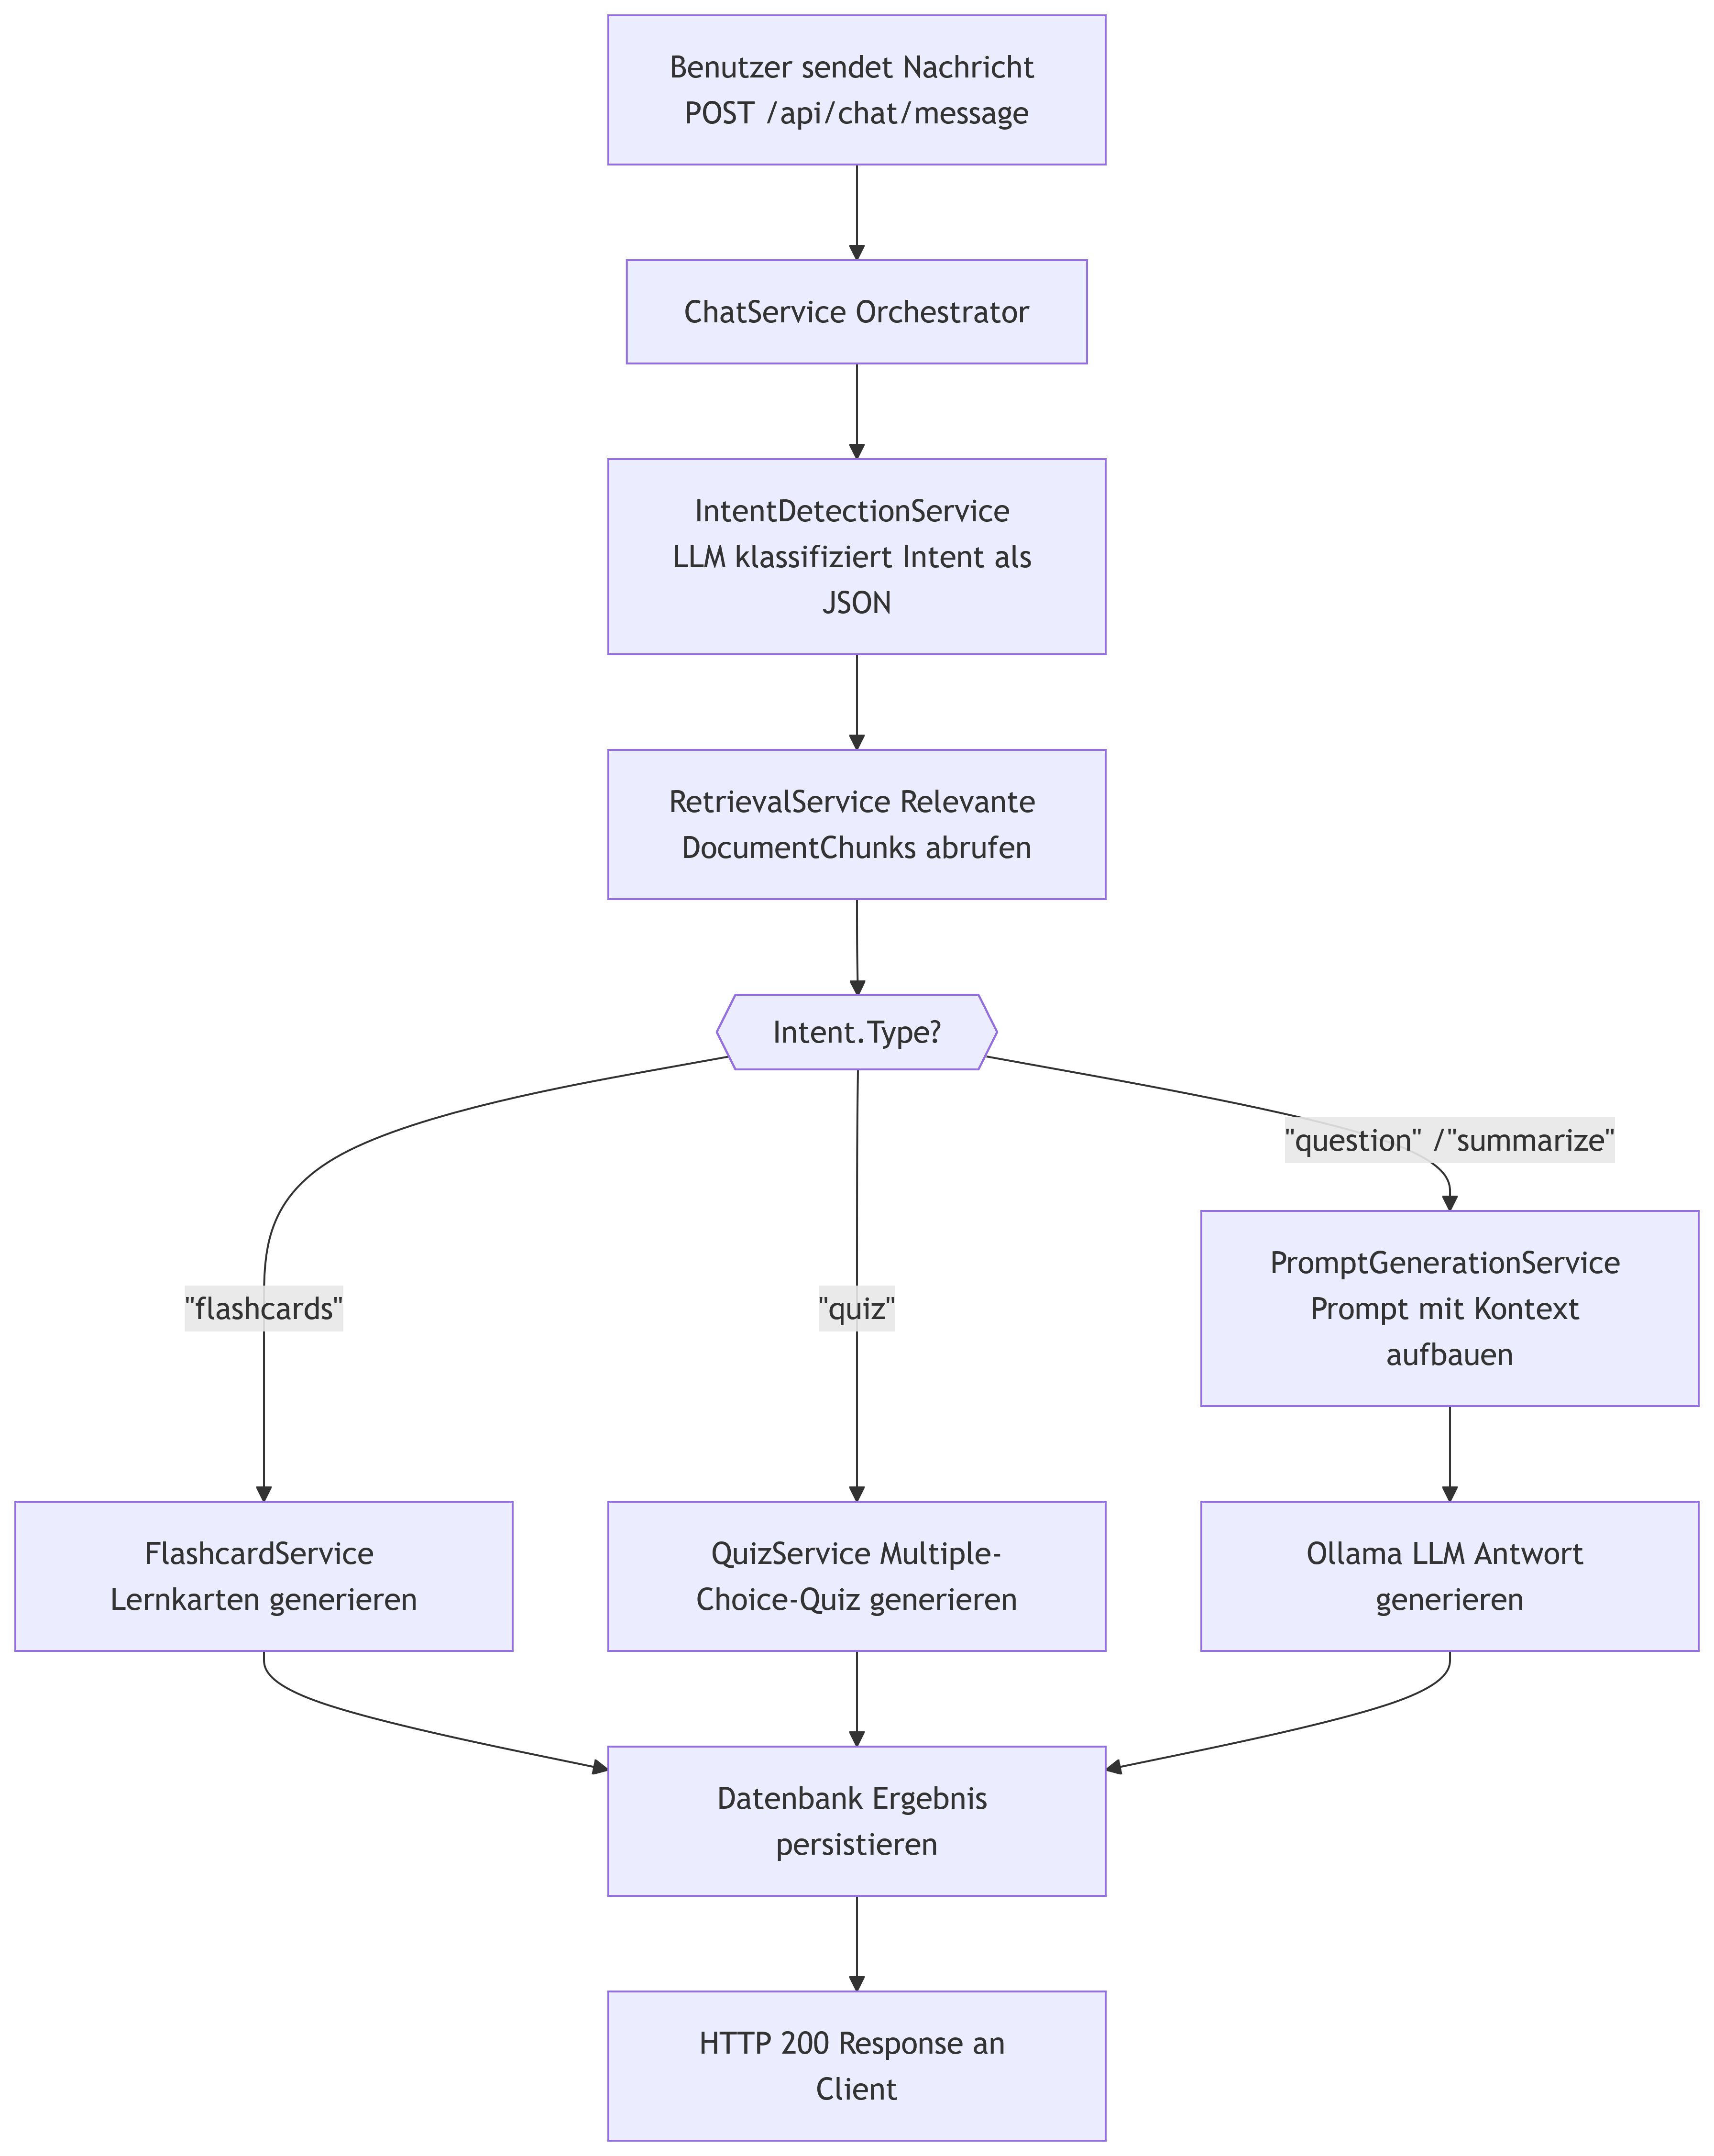
\includegraphics[width=\textwidth]{img/intent_branching.png}
    \caption{Intent-basiertes Branching im ChatService}
    \label{fig:intent_branching}
\end{figure}

\subsection{Schritt 4: Orchestrierung und Intent-basiertes Branching (\texttt{ChatService})}
\label{subsec:chatservice}

Der \texttt{ChatService} fungiert als zentraler Orchestrator und trifft nach der Retrieval-Phase eine \textbf{Intent-basierte Fallunterscheidung}. Dies unterscheidet EduShelf von einem einfachen Chatbot:

\begin{lstlisting}[language={[Sharp]C}, caption={Intent-basiertes Branching in ChatService.cs}]
var intent = await _intentDetectionService.GetIntentAsync(promptInput);
var relevantChunks = await _retrievalService.GetRelevantChunksAsync(
    promptInput, userId, intent);

if (intent.Type == "flashcards") {
    await _flashcardService.GenerateFlashcardsAsync(
        new GenerateFlashcardsRequest { Context = context, Count = 5 }, userId);
    responseContent = "I have generated flashcards.";
}
else if (intent.Type == "quiz") {
    await _quizService.GenerateQuizAsync(
        new GenerateQuizRequest { Context = context, Count = 5 }, userId);
    responseContent = "I have generated a quiz.";
}
else { // "question" oder "summarize"
    var chatHistory = _promptGenerationService.BuildChatHistory(
        chatSession, relevantChunks, promptInput);
    var result = await chatCompletionService.GetChatMessageContentAsync(chatHistory);
    responseContent = result.Content ?? "Sorry, no response generated.";
}
\end{lstlisting}

Dieses Design erm\"oglicht es, \"uber eine einzige Chat-Schnittstelle drei fundamentale Lernfunktionen anzubieten: konversationelles Frage-Antwort, automatische Flashcard-Generierung und automatische Quiz-Erstellung, alles gesteuert durch die Intention hinter der sprachlichen Eingabe des Nutzers.

\subsection{Zusammenfassung: Retrieval-Augmented Generation}
Die Implementierung des RAG-Systems stellt sicher, dass das LLM stets auf den spezifischen Kontext der hochgeladenen Dokumente des Nutzers antwortet. Die wichtigsten Designprinzipien sind:
\begin{itemize}
    \item \textbf{Datenprivacy:} Durch den lokalen Ollama-Server verlassen keine Dokumenteninhalte den Server.
    \item \textbf{Pr\"azision:} Durch semantische Vektorsuche und optionales Name-Matching werden nur die relevantesten Chunks an das LLM \"ubergeben.
    \item \textbf{Robustheit:} Token-basierte Kontextlimitierung verhindert LLM-Abst\"urze durch \"uberlange Prompts.
    \item \textbf{Erweiterbarkeit:} Das Intent-Branching erlaubt es, neue KI-gest\"utzte Features durch Hinzuf\"ugen weiterer Intent-Typen zu integrieren, ohne die Pipeline zu \"andern.
\end{itemize}
